\documentclass{article}

%<importy paczek>
\usepackage[utf8]{inputenc}
\usepackage[margin=3cm]{geometry}
\usepackage{graphicx}
\usepackage{xcolor}
\usepackage{titlesec}
\usepackage{tabularray}
\usepackage{float}
\usepackage{url}
\usepackage[breaklinks]{hyperref}
\hypersetup{
    colorlinks=true,
    linkcolor=black,
    urlcolor=blue,
}
\definecolor{pinkish}{RGB}{165, 107, 142}
\titlespacing*{\section}
{0pt}{9ex}{5ex}



\title{\Huge\textbf{\color{pinkish}Predicting the cause of death based on age and musical skill} \\
    \LARGE \textbf{{System Analysis and Decision Support Methods}}}
\author{
    Natalia Malinowska \\
    272669 \\
    Applied Computer Science \\
    Wroclaw University of Science and Technology\\
    Wed. (even) 15:15
}
\date{10th of June 2024}


\begin{document}


\begin{titlepage}
    \maketitle
    \thispagestyle{empty} 
\end{titlepage}

\tableofcontents


\clearpage
\section{Problem intro}

The problem addressed in the research is the relationships between data on deceased musicians, including the causes of their deaths. The inspiration for these considerations was asking whether it is possible to effectively predict what a musician will die from, taking into account factors such as their age, place of residence, genre of music played, or musical skills.

The aim of this study is to analyze whether this data can be used to build a predictive model for the causes of death among musicians. By analyzing the acquired dataset, patterns and correlations are sought that may provide information on how these factors interact, and potentially influence the mortality of musicians. We will use various statistical methods to analyze the data, conduct experiments on them, and create a model.

The assumption is that there is some relationship between the deaths of musicians and the genre of music they engage in. For example, musicians performing hip hop or rock music are known for a more impulsive, risky lifestyle than jazz or classical musicians - therefore, such a relationship should emerge from our considerations.


\section{Dataset acquisition and exploratory analysis}


\subsection{Dataset acquisition}

Acquiring complete, reliable data, then cleaning, and preparing it for analysis, was likely the most challenging task in this project.

The initial dataset of deceased artists was obtained from the \textit{rateyourmusic.com} website using web scraping method with the help of the \textit{BeautifulSoup} Python library. However, there was a lack of data about artists' birth dates – necessary for calculating their age – as well as several parameters that could potentially be used for additional analysis, such as gender or music genre. To address this, an API provided by the \textit{musicbrainz.org} website was utilized.

After obtaining two datasets, they were synthesized into one dataset by matching them based on the artists' names. Then, a multi-stage process of data cleaning and preparation was carried out. The age was calculated, the places of residence were shortened (to countries only), and the data was generalized – for example, nearly 200 causes of death that came in various forms were categorized into 11 categories, similarly done with music genres, and skills.


\subsubsection{Individual stages of data acquisition and processing}
\begin{enumerate}
\item[a)] Obtaining the first part of the data using a web scraping method
\item[b)] Obtaining the second part of the data using an API method
\item[c)] Data synthesis
\item[d)] Standardization of data
\item[e)] Removal of erroneous and empty data
\item[f)] Generalization/categorization of data
\item[g)] Repairing data formatting errors
\item[h)] Generating separate datasets (non-atomic data in columns, e.g., "piano, guitar, vocals" in the "musical\_skills" column, were split into atomic values to enable proper analysis)
\end{enumerate}



\clearpage
\subsection{Exploratory analysis of the dataset}


\subsubsection{Analysis of the amount of deaths within a particular parameter}

\begin{figure}[H]
    \centering
    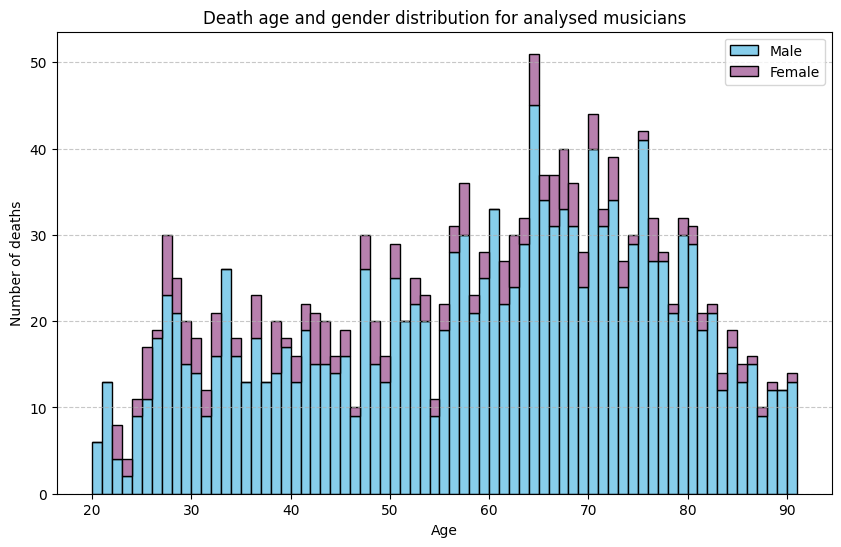
\includegraphics[width=0.8\linewidth]{graph_images/exploratory_analysis/age_gender.png}
    \label{fig:enter-label}
\end{figure}

\begin{figure}[H]
    \centering
    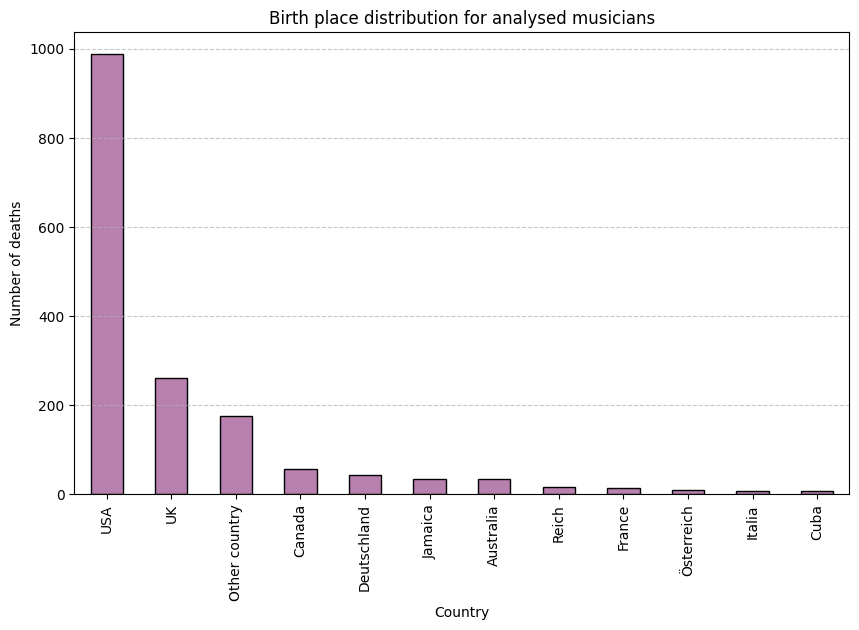
\includegraphics[width=0.8\linewidth]{graph_images/exploratory_analysis/birthplace.png}
    \label{fig:enter-label}
\end{figure}

\begin{figure}[H]
    \centering
    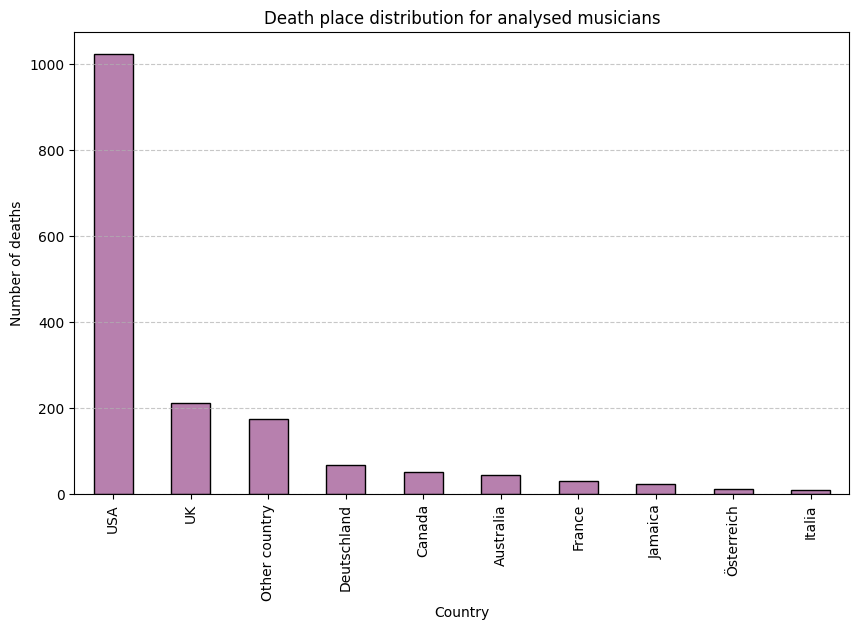
\includegraphics[width=0.8\linewidth]{graph_images/exploratory_analysis/deathplace.png}
    \label{fig:enter-label}
\end{figure}

\begin{figure}[H]
    \centering
    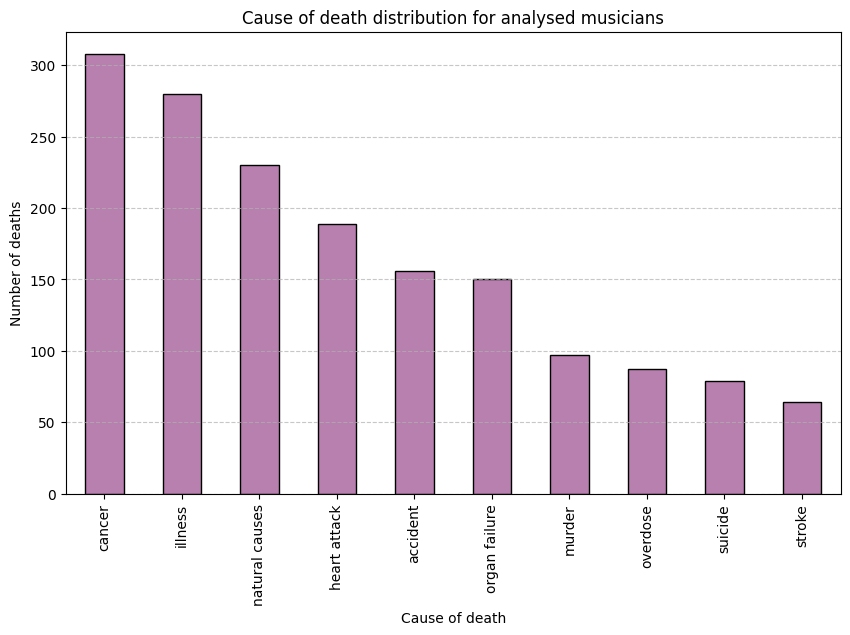
\includegraphics[width=0.8\linewidth]{graph_images/exploratory_analysis/deathcause.png}
    \label{fig:enter-label}
\end{figure}

\begin{figure}[H]
    \centering
    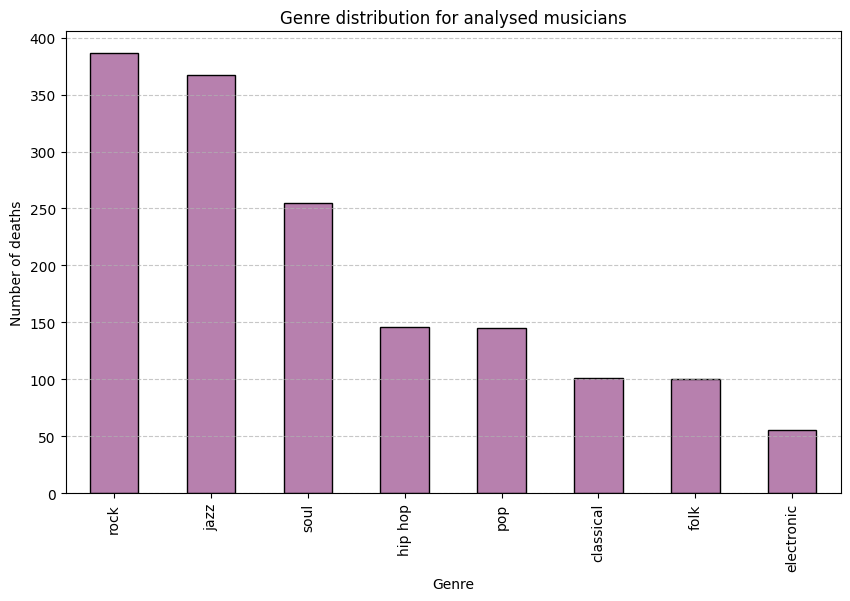
\includegraphics[width=0.8\linewidth]{graph_images/exploratory_analysis/genre.png}
    \label{fig:enter-label}
\end{figure}

\begin{figure}[H]
    \centering
    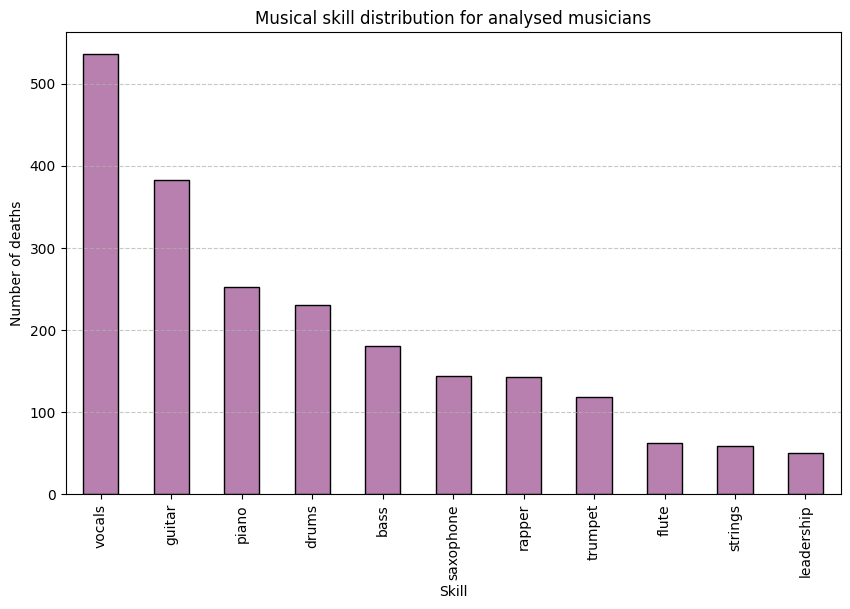
\includegraphics[width=0.8\linewidth]{graph_images/exploratory_analysis/skill.png}
    \label{fig:enter-label}
\end{figure}



\subsubsection{Individual cause of death analysis}

\begin{figure}[H]
    \centering
    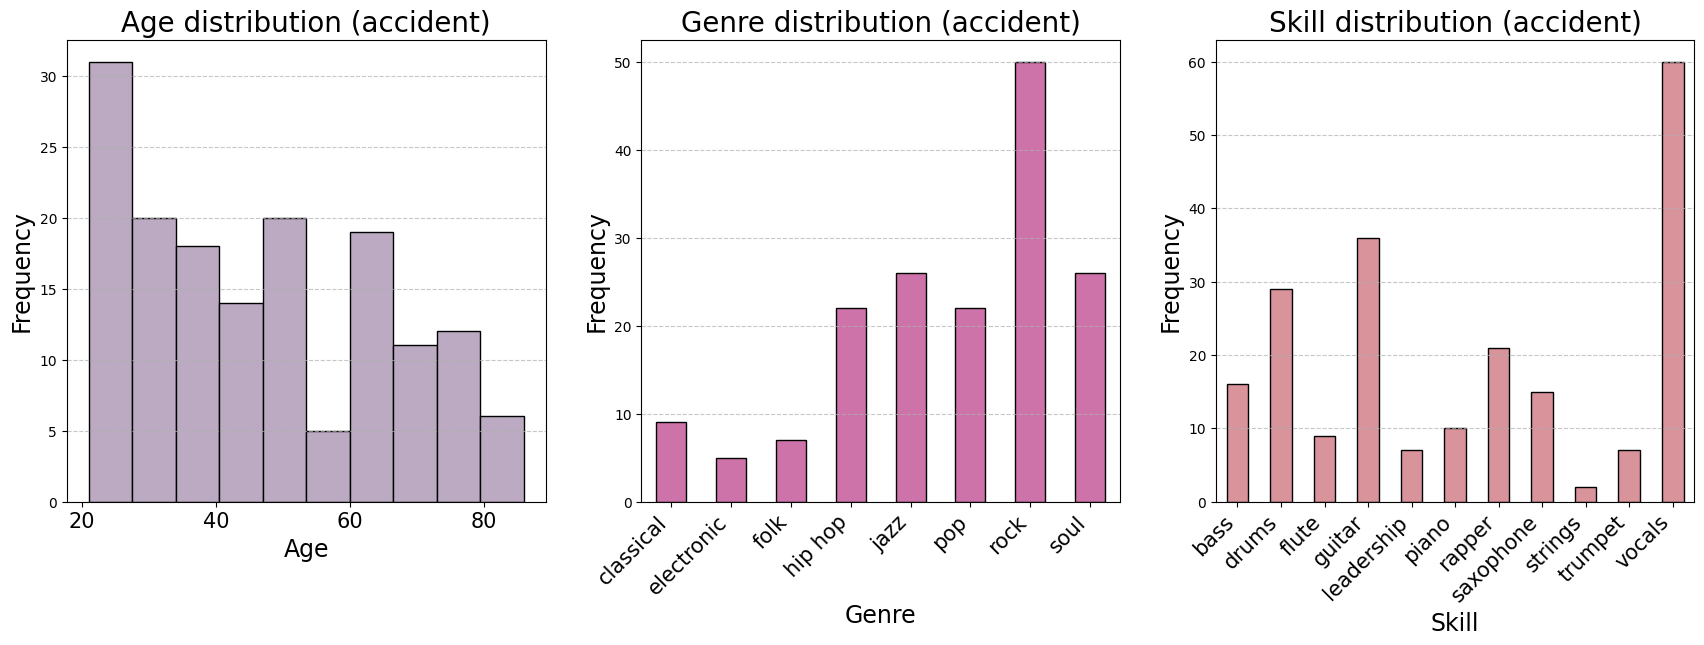
\includegraphics[width=1\linewidth]{graph_images/death_cause_analysis/accident_distribution.png}
    \label{fig:enter-label}
\end{figure}

\begin{figure}[H]
    \centering
    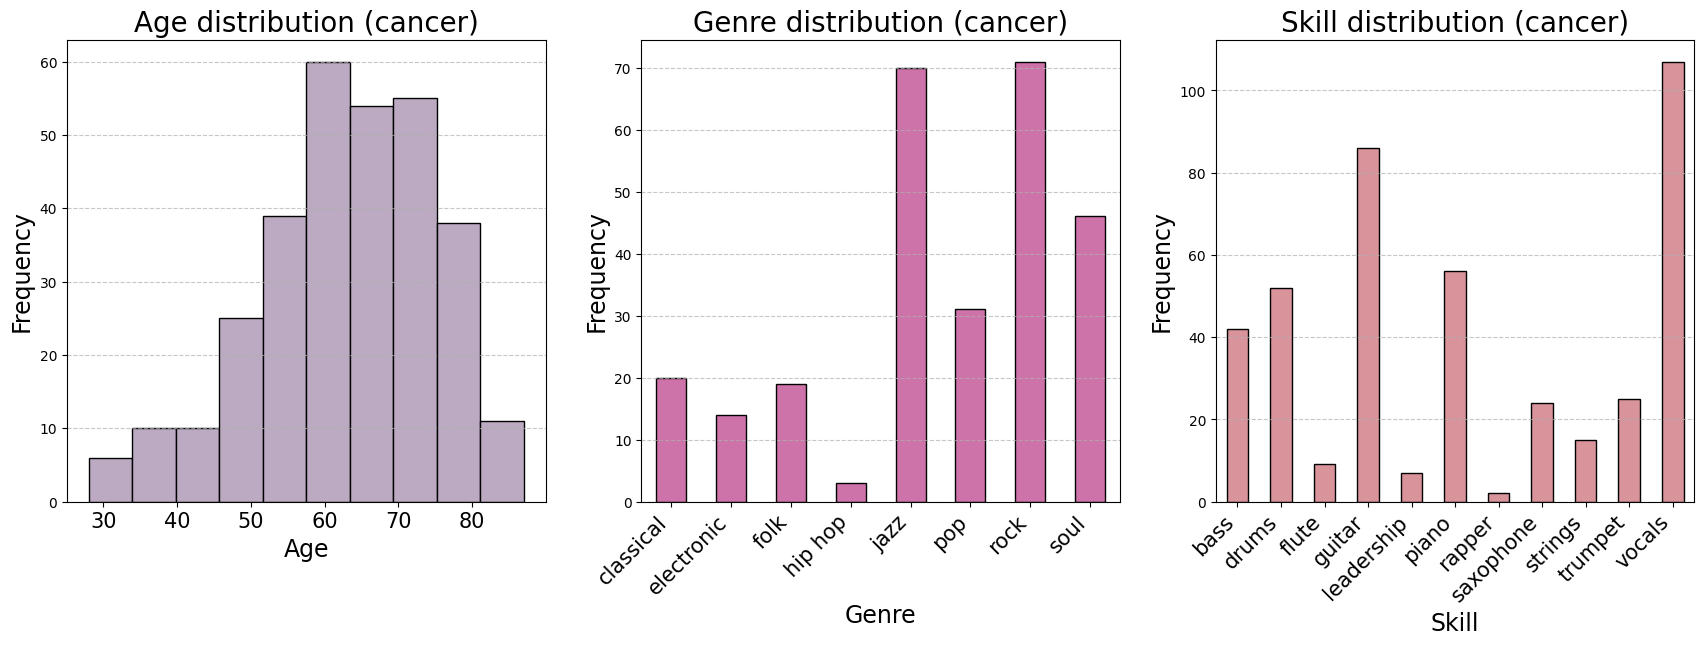
\includegraphics[width=1\linewidth]{graph_images/death_cause_analysis/cancer_distribution.png}
    \label{fig:enter-label}
\end{figure}

\begin{figure}[H]
    \centering
    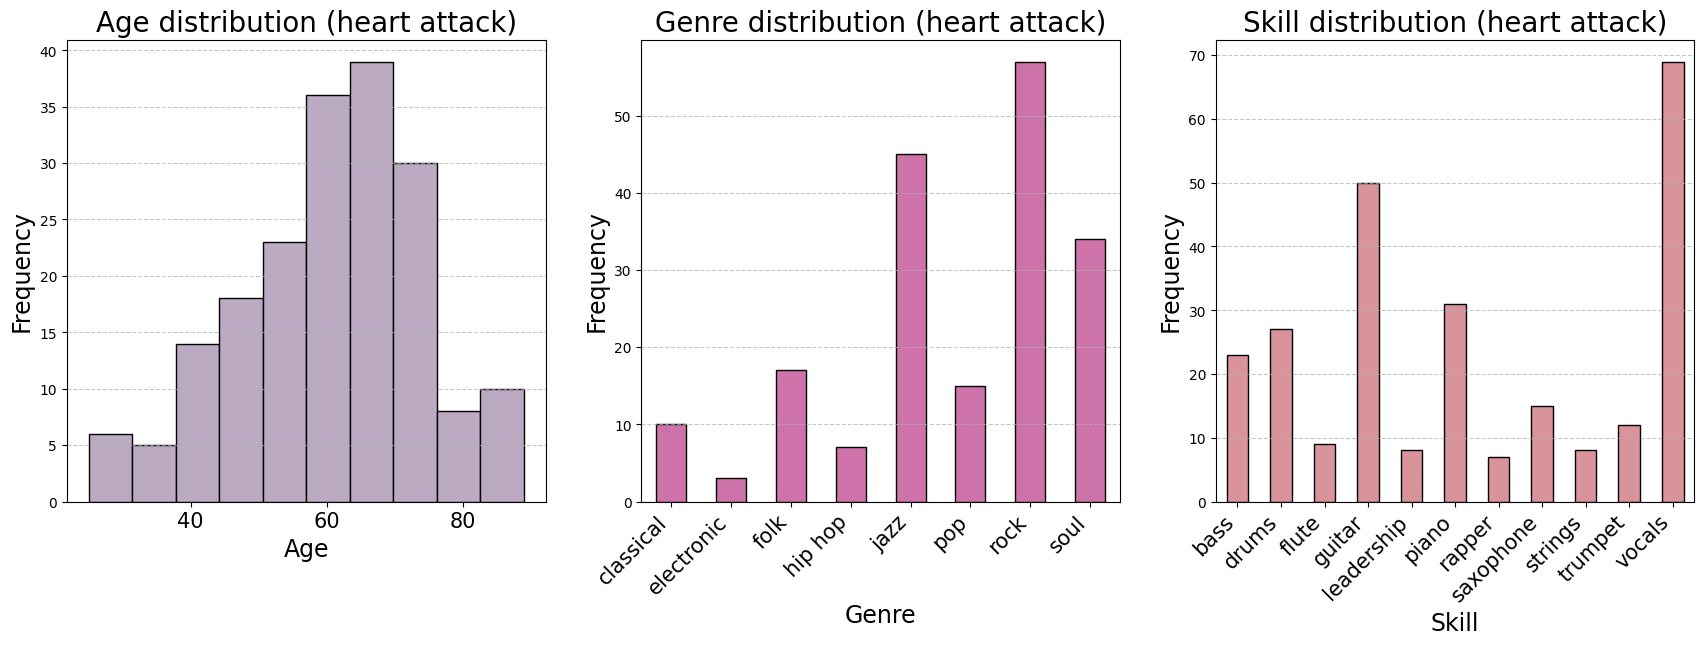
\includegraphics[width=1\linewidth]{graph_images/death_cause_analysis/heart_attack_distribution.png}
    \label{fig:enter-label}
\end{figure}

\begin{figure}[H]
    \centering
    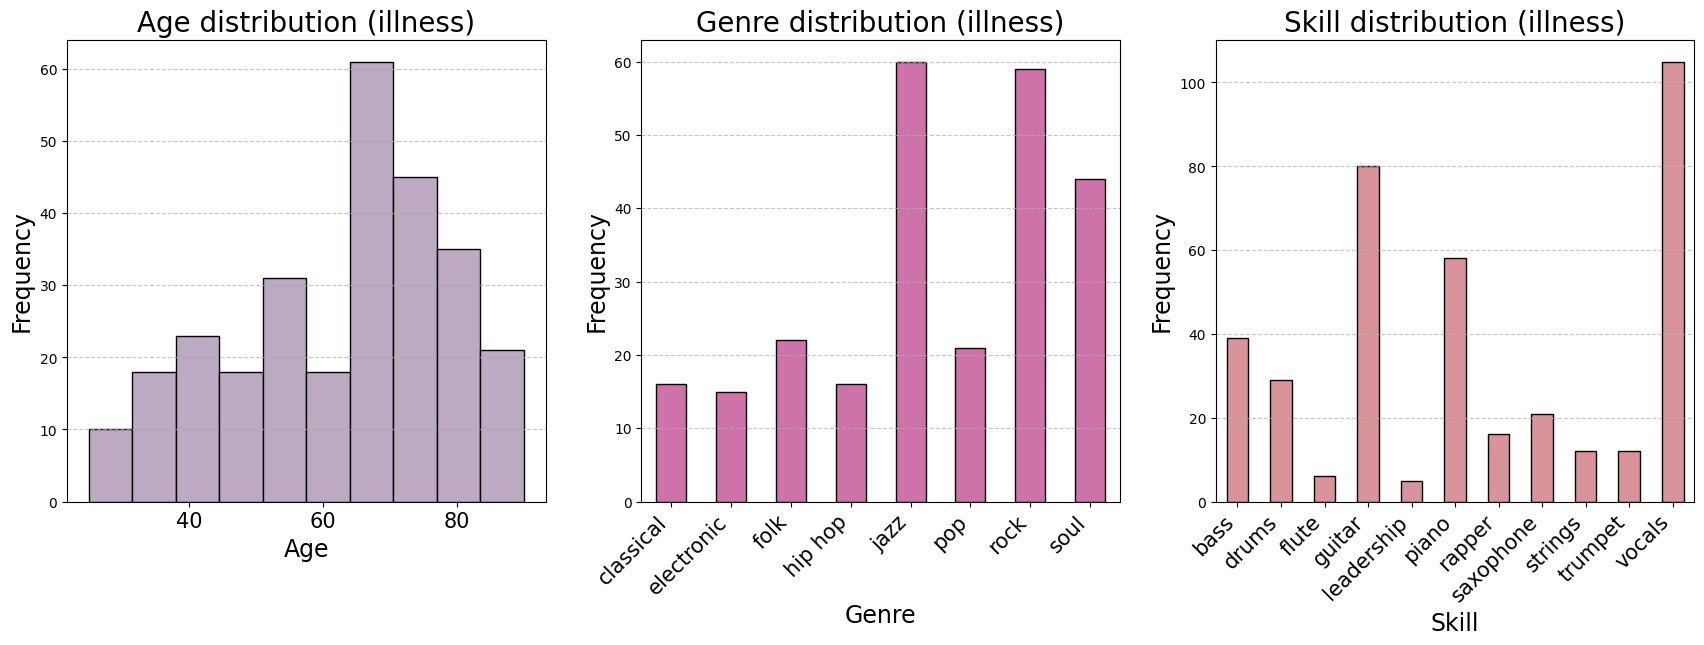
\includegraphics[width=1\linewidth]{graph_images/death_cause_analysis/illness_distribution.png}
    \label{fig:enter-label}
\end{figure}

\begin{figure}[H]
    \centering
    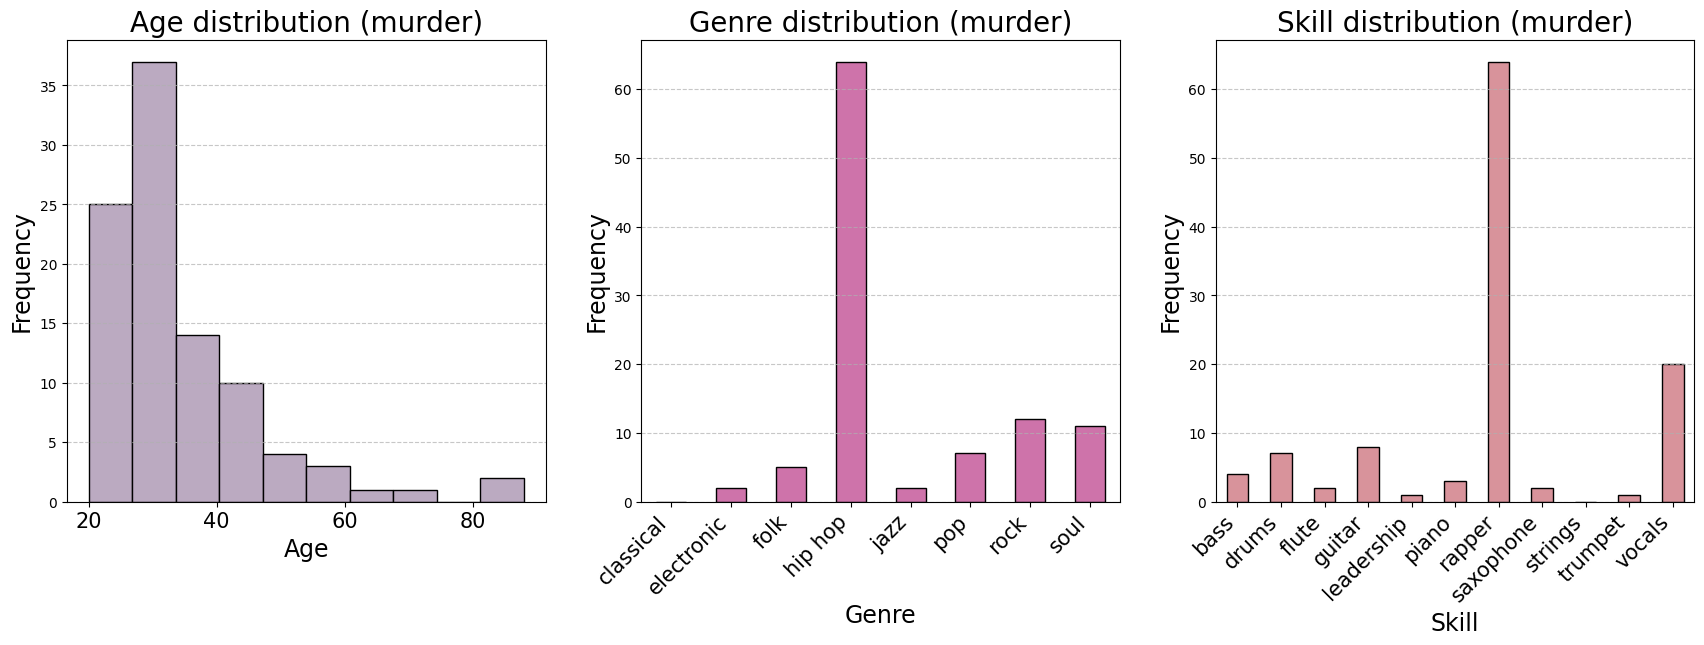
\includegraphics[width=1\linewidth]{graph_images/death_cause_analysis/murder_distribution.png}
    \label{fig:enter-label}
\end{figure}

\begin{figure}[H]
    \centering
    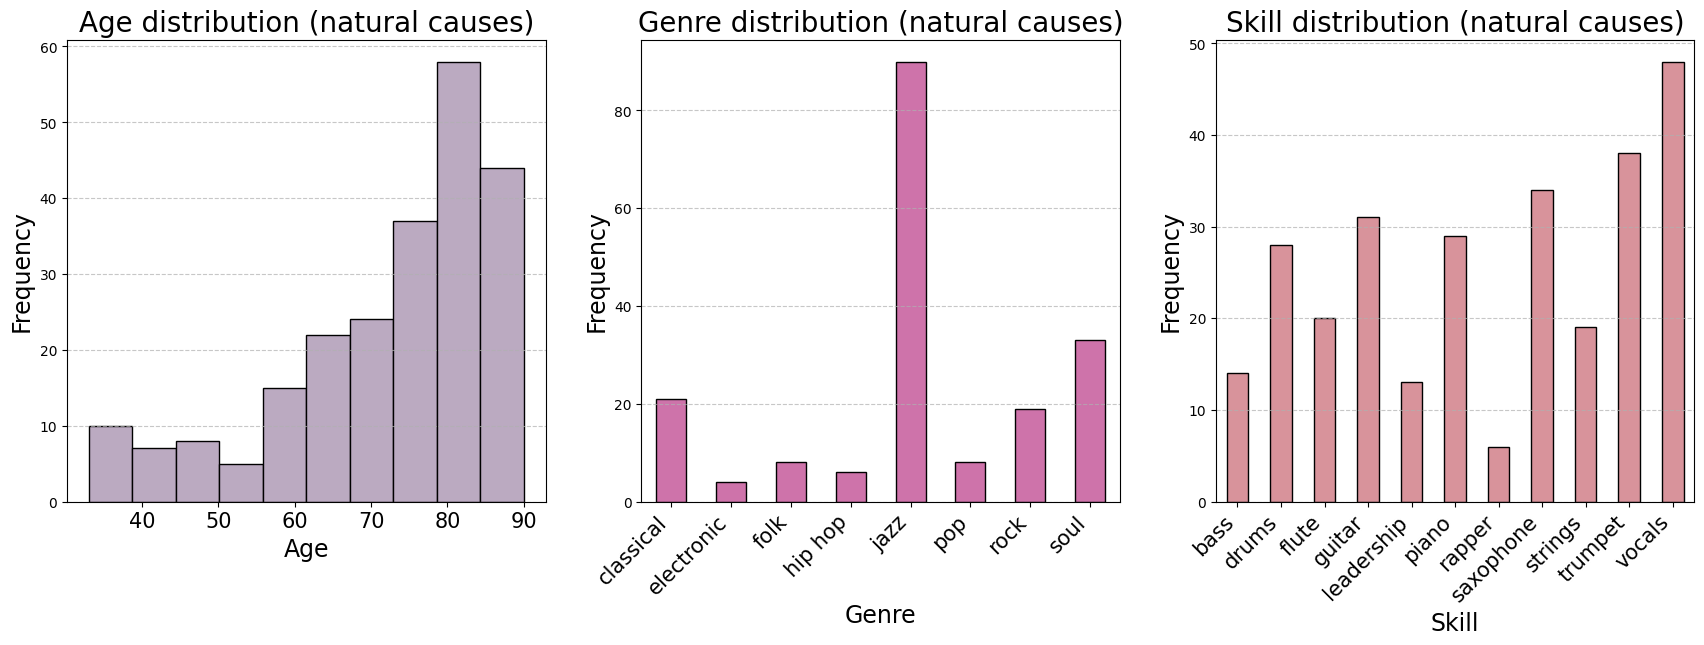
\includegraphics[width=1\linewidth]{graph_images/death_cause_analysis/natural_causes_distribution.png}
    \label{fig:enter-label}
\end{figure}

\begin{figure}[H]
    \centering
    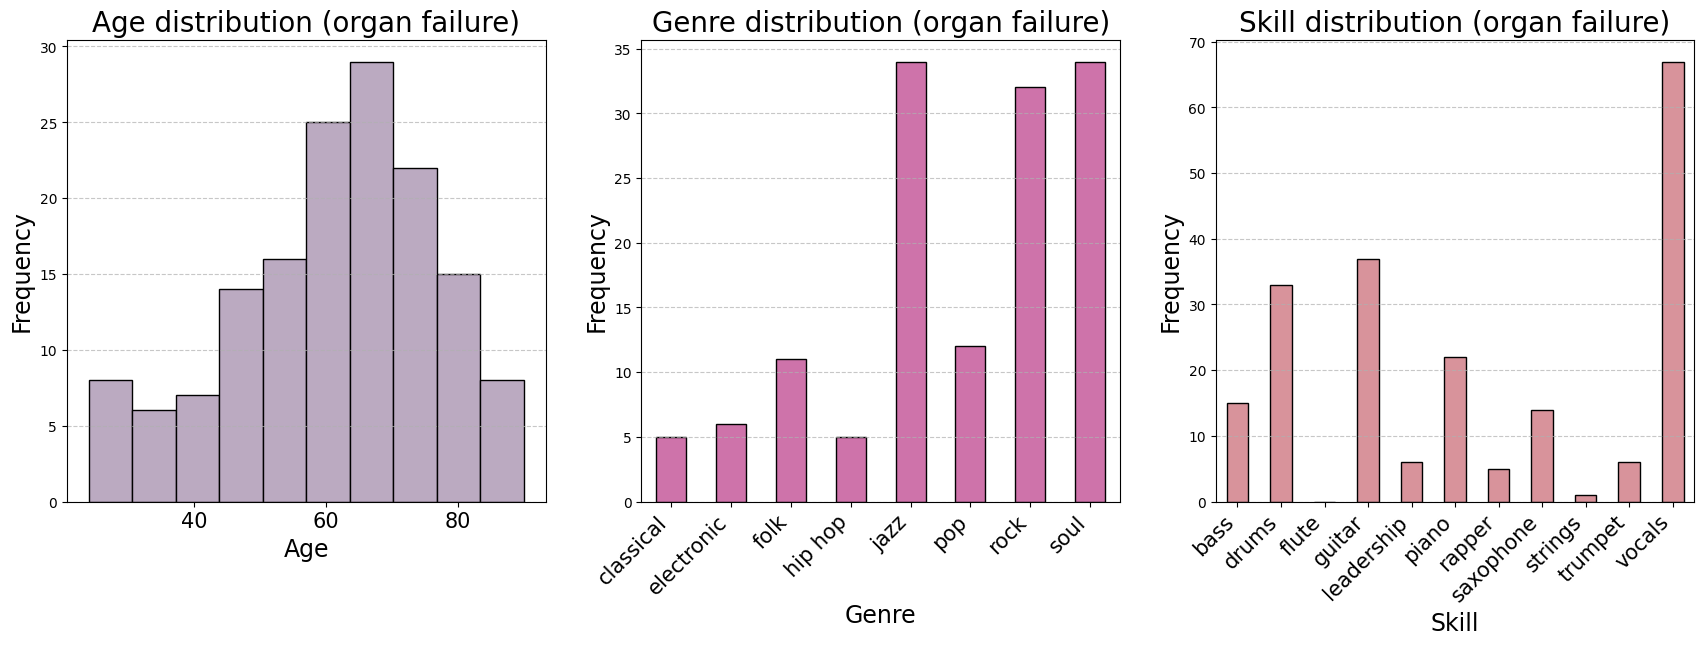
\includegraphics[width=1\linewidth]{graph_images/death_cause_analysis/organ_failure_distribution.png}
    \label{fig:enter-label}
\end{figure}

\begin{figure}[H]
    \centering
    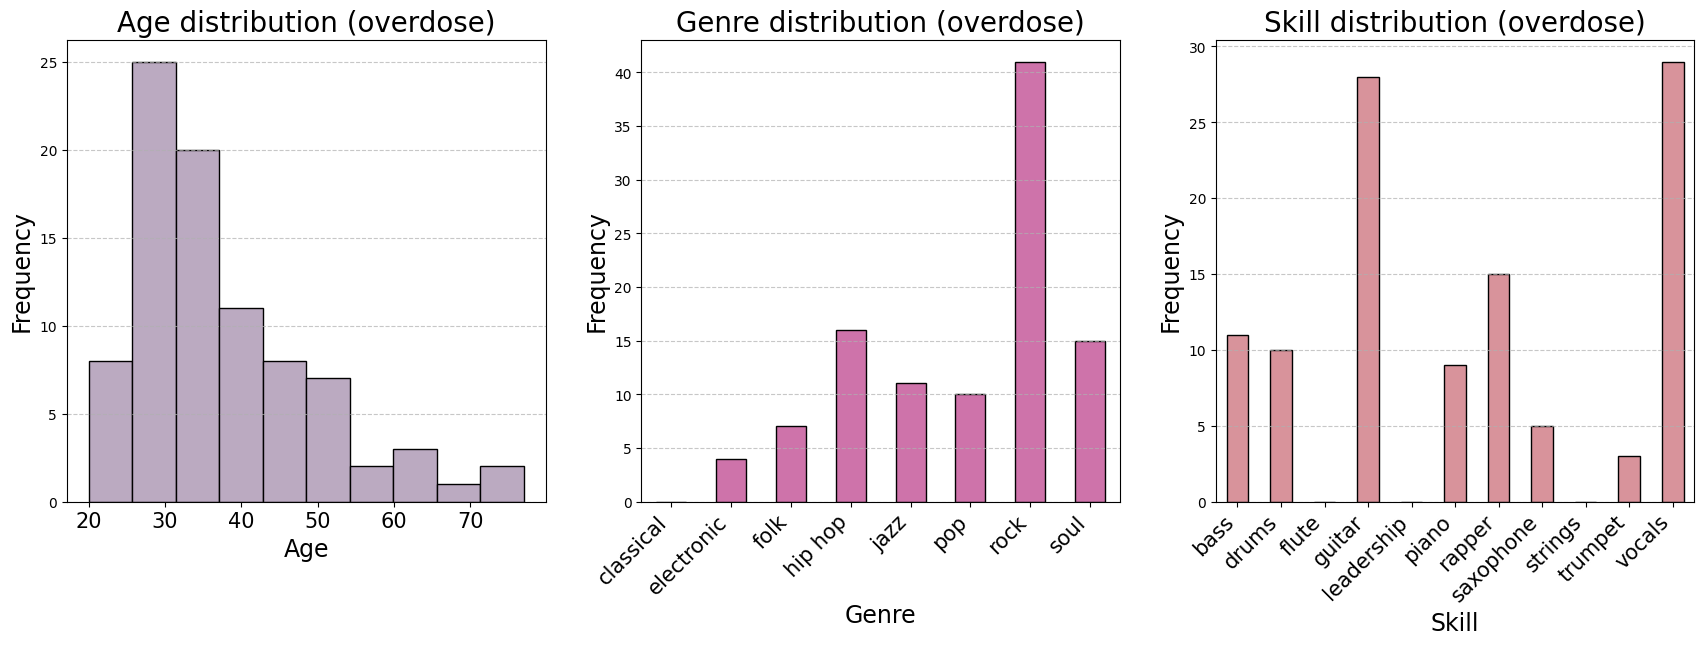
\includegraphics[width=1\linewidth]{graph_images/death_cause_analysis/overdose_distribution.png}
    \label{fig:enter-label}
\end{figure}

\begin{figure}[H]
    \centering
    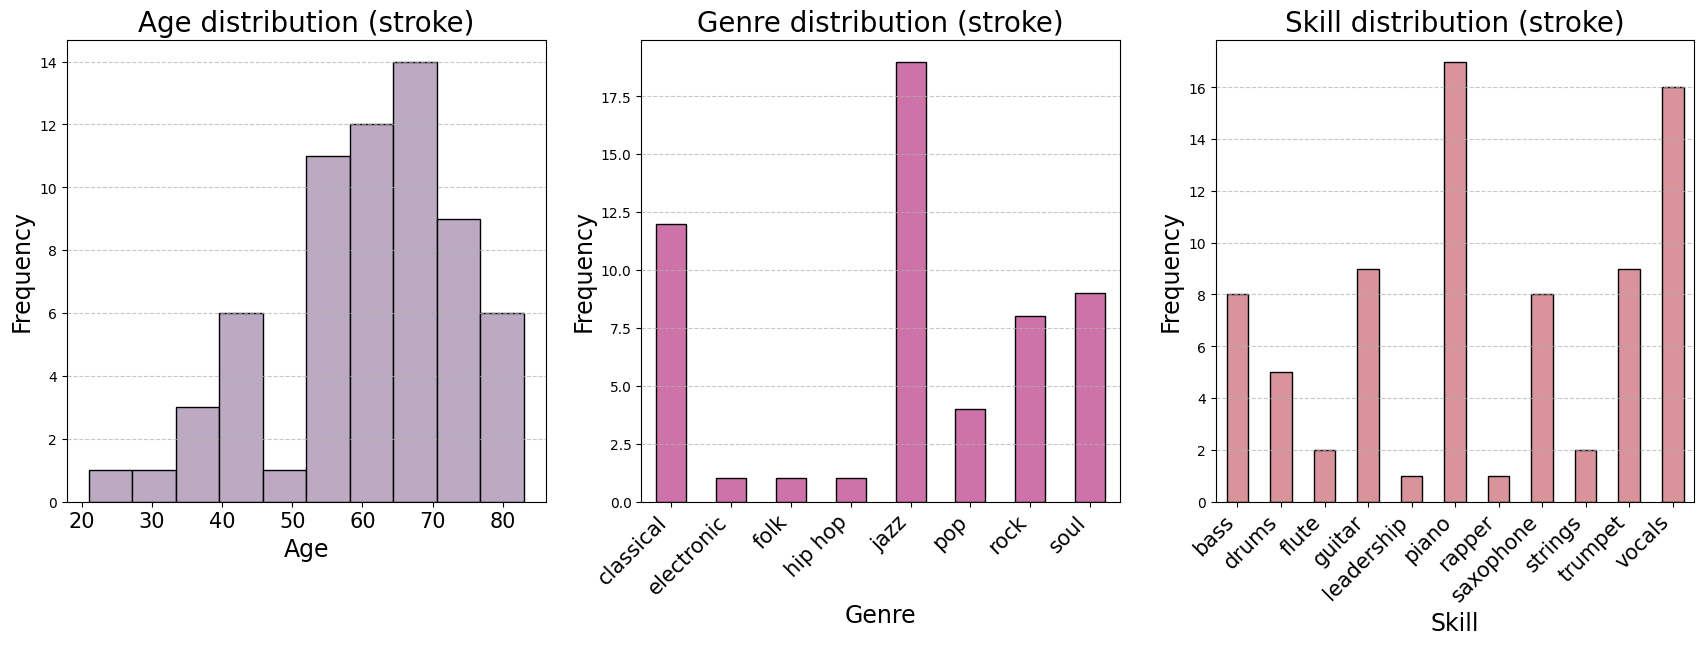
\includegraphics[width=1\linewidth]{graph_images/death_cause_analysis/stroke_distribution.png}
    \label{fig:enter-label}
\end{figure}

\begin{figure}[H]
    \centering
    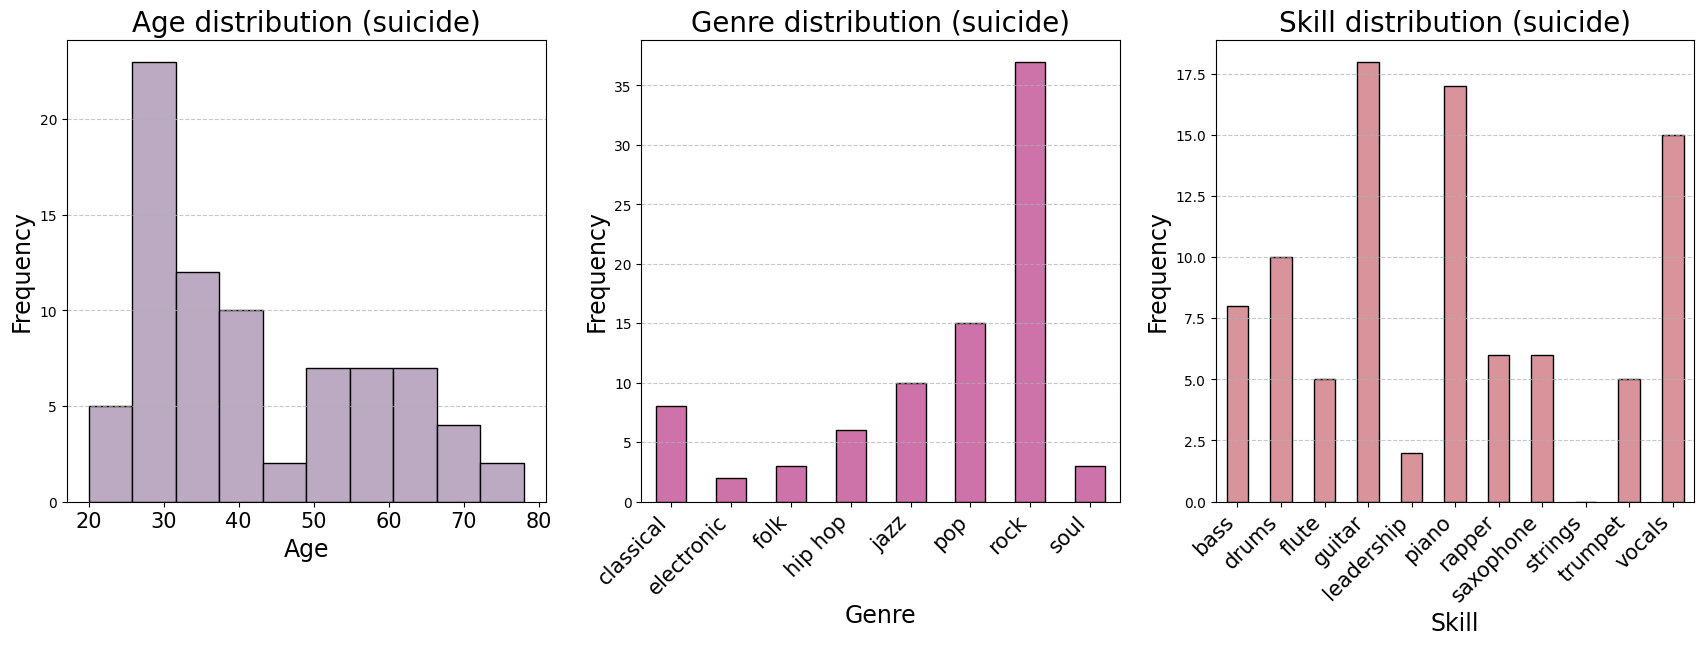
\includegraphics[width=1\linewidth]{graph_images/death_cause_analysis/suicide_distribution.png}
    \label{fig:enter-label}
\end{figure}



\subsection{Characteristics of the dataset and conclusions}

Analyzing the data led to the decision to specify the following parameters:
\begin{itemize}
    \item {\textit{age}} - ranged 20-100
    \item {\textit{birth\_place}} - primarily USA and UK
    \item {\textit{death\_place}} - primarily USA and UK
    \item {\textit{cause\_of\_death}} - 10 categories: cancer, illness, natural causes, heart attack, organ failure, accident, murder, overdose, suicide, stroke
    \item {\textit{musical\_skills}} - 11 categories: vocals, guitar, piano, drums, bass, saxophone, rapper, trumpet, flute, strings, leadership
    \item {\textit{genres}} - 8 categories: rock, jazz, soul, pop, hip hop, folk, electronic, classical
\end{itemize}

After conducting the data exploration, the data on the gender and birth/death locations of the artists had to be discarded during the further analysis. Unfortunately, despite efforts, the acquired dataset predominantly consisted of males (approx. 80\% of the data) and artists residing in the USA (approx. 70\% of the data). Such an imbalance in the data would not lead to any meaningful results; consequently, these parameters were omitted from the final analysis.

It is worth mentioning that due to the lack of data, not every musician is provided with a genre. It has led to creating a separate dataset, consisting of around 1300 records - it is smaller than the original dataset, consisting of around 2000 records after separating data (point h. mentioned in the data acquisition process).



\clearpage
\section{Experiments}


\subsection{Correlation matrices}

The following heatmaps showcase the correlation between the amount of deaths in certain age groups and chosen parameters.

It is important to mention that the counts have been normalised to make up for the data imbalances, by dividing the total amount of the deaths by the given cause (as discovered in the exploratory analysis, there is - for example - much more data on certain death causes, leading to the impairment of the credibility of the results).

\begin{figure} [H]
    \centering
    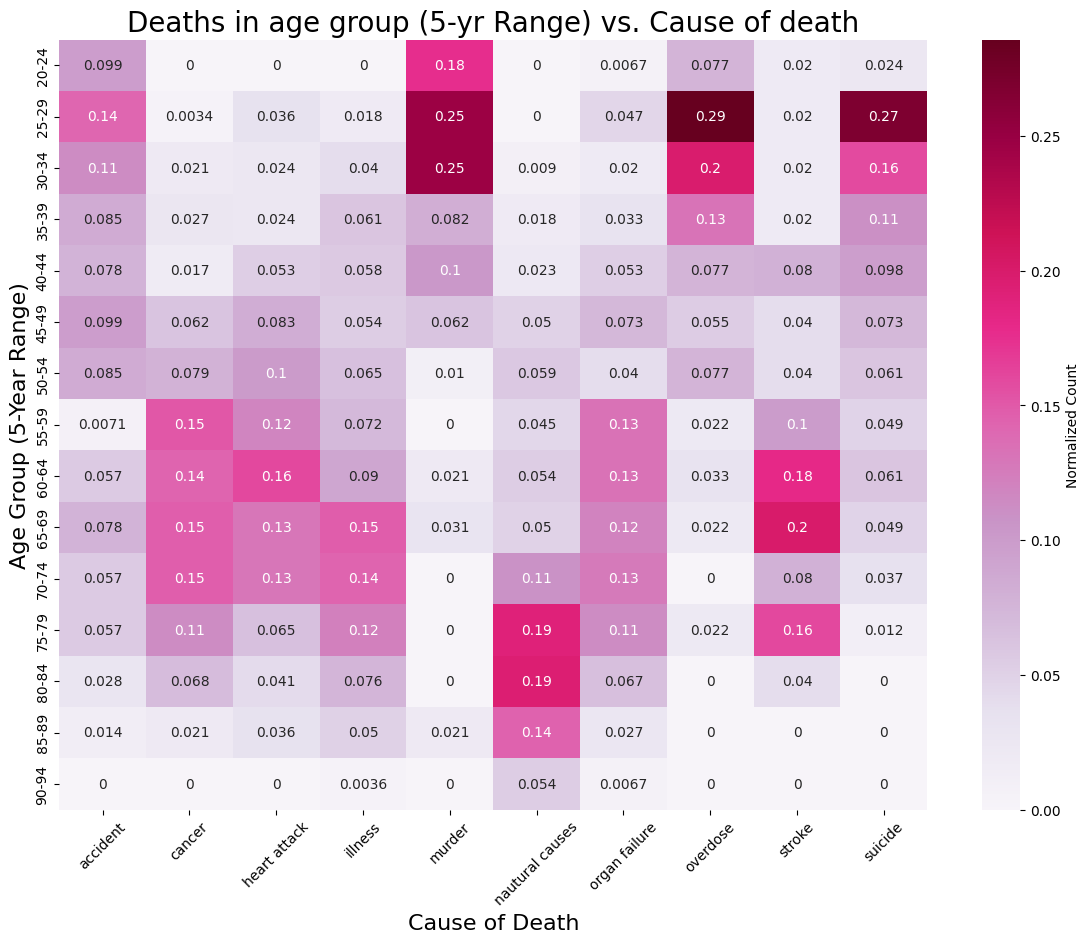
\includegraphics[width=1\linewidth]{graph_images/heatmaps/age vs death cause.png}
    \label{fig:enter-label}
\end{figure}

Despite the limitations of the dataset, we can clearly see some patterns forming already - for example, deaths by natural causes occurring primarily in older age groups, whereas deaths by overdose, suicide or murder tend to occur within younger age groups.

\begin{figure} [H]
    \centering
    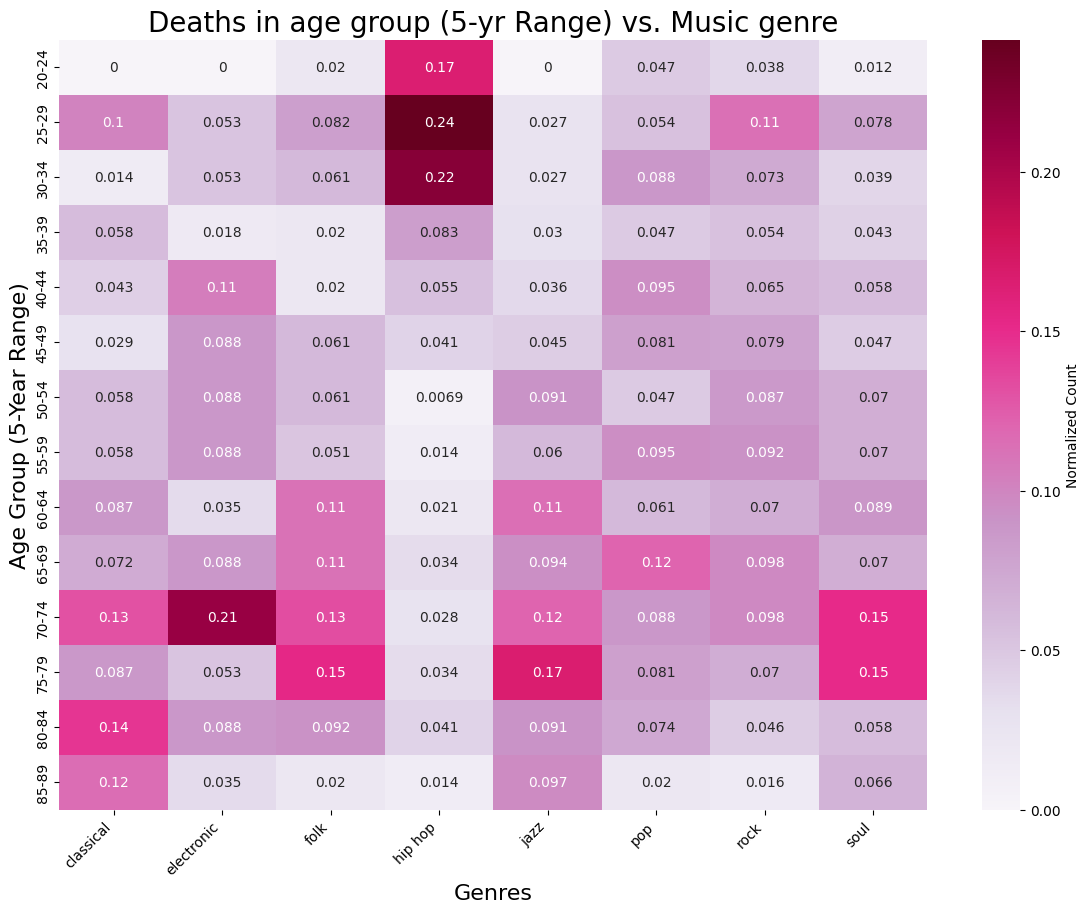
\includegraphics[width=1\linewidth]{graph_images/heatmaps/age vs genre.png}
    \label{fig:enter-label}
\end{figure}

Although not too dependable, some correlations can be observed - for example, musicians performing "calmer", more sophisticated genres tend to live longer lives, whereas rappers or rock stars on average have shorter lifespans, most likely due to their unhealthy, more impulsive lifestyles.

\begin{figure} [H]
    \centering
    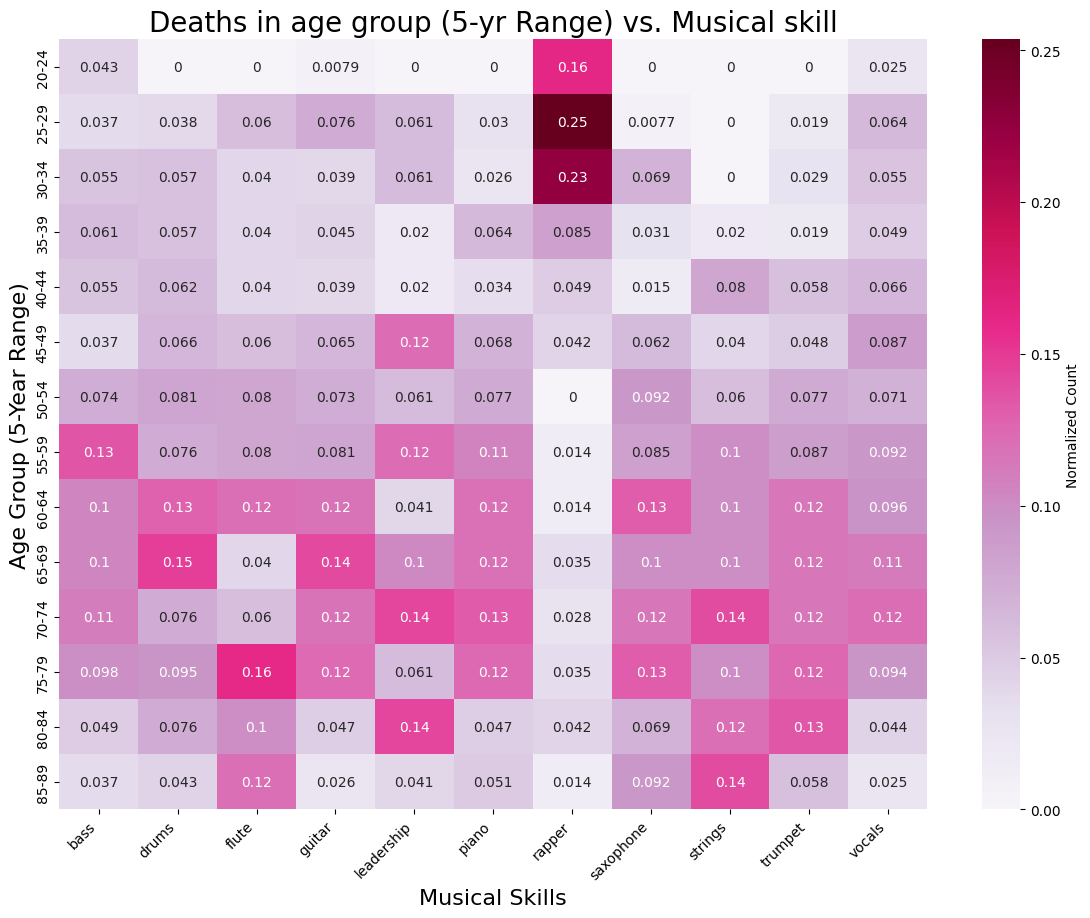
\includegraphics[width=1\linewidth]{graph_images/heatmaps/age vs musical skill.png}
    \label{fig:enter-label}
\end{figure}

In this heatmap we can see the clear dataset bias towards rappers who have died at a young age. Some correlations can be observed, but it seems obvious that more high-quality data is needed to draw better conclusions, more rooted in reality.


\begin{figure} [H]
    \centering
    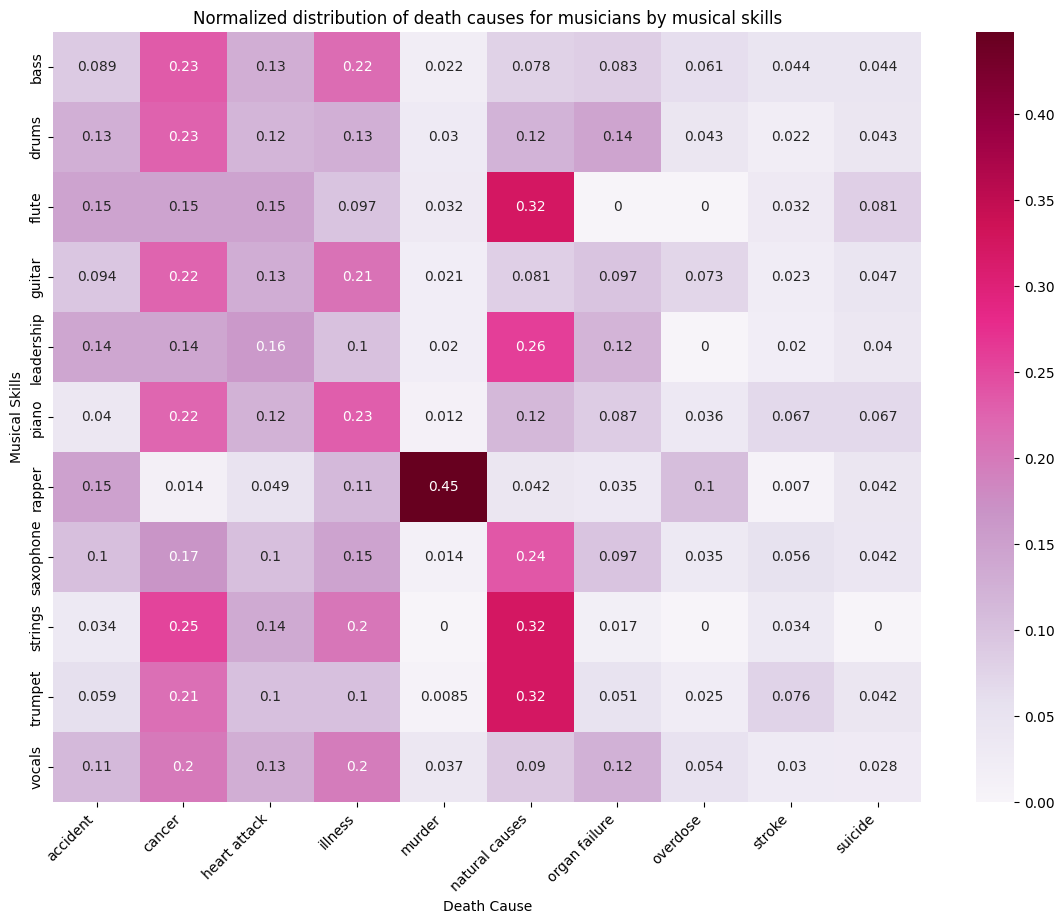
\includegraphics[width=1\linewidth]{graph_images/heatmaps/heatmapextra.png}
    \label{fig:enter-label}
\end{figure}

Here we see another clear example of dataset bias, particularly within the murder category.



\clearpage
\subsection{Linear and polynomial regression}

While trying to fit the regression models to the datasets, the train/test split has been taken with a test\_size of 0.2 (the models have been trained on 80\% of data and tested on the remaining 20\% of them).

The first trial of fitting a regression model to the dataset ended up in a failure. The data was too scattered. As a result, the results of the adopted performance indicators - Root Mean Squared Error and R\textasciicircum2 score - were extremely low and therefore unsatisfying.

The results of the original trial are as follows:

\begin{figure} [H]
    \centering
    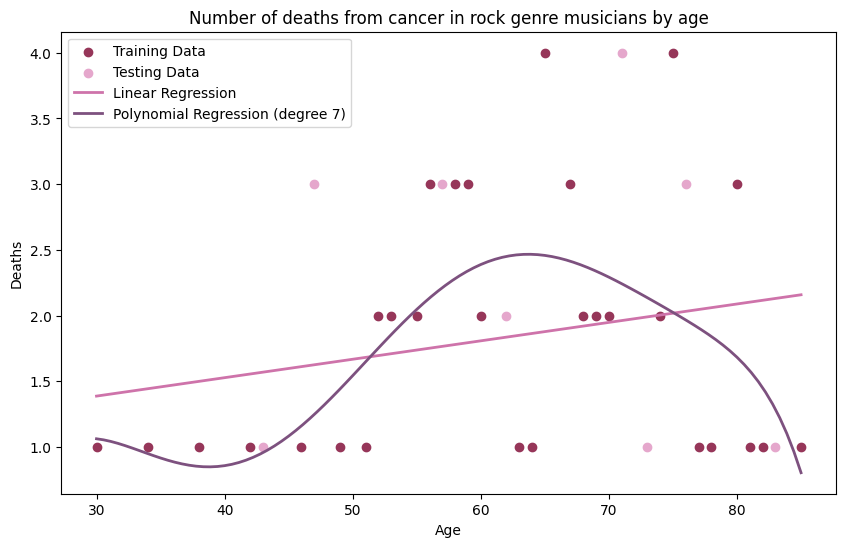
\includegraphics[width=0.6\linewidth]{graph_images/experiments/failed.png}
    \label{fig:enter-label}
\end{figure}

\noindent\texttt{Linear Regression - Training Set: RMSE = 0.9269, R\textasciicircum2 = 0.0467\\
Linear Regression - Testing Set: RMSE = 1.1785, R\textasciicircum2 = -0.1697\\
Polynomial Regression - Training Set: RMSE = 0.7817, R\textasciicircum2 = 0.322\\
Polynomial Regression - Testing Set: RMSE = 1.0855, R\textasciicircum2 = 0.0078\\}


Further explorations have led to grouping the data into ranges - taking a sum of deaths for every 5-year range. This has led to a much better fitting of the models, and therefore the performance indicators returned a much more satisfactory results, presented below.

Only a few combinations of death causes, genres and skills were chosen for demonstration purposes.



\subsubsection{Fitting a linear regression model and a polynomial regression of degree n to the data: death cause - cancer, genre - rock}

\begin{figure} [H]
    \centering
    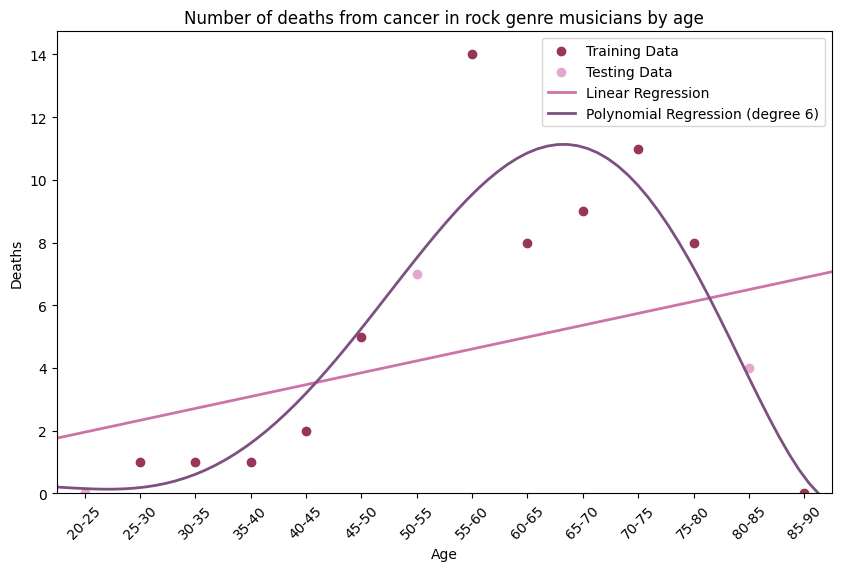
\includegraphics[width=0.6\linewidth]{graph_images/experiments/exp1.png}
    \label{fig:enter-label}
\end{figure}

\noindent\texttt{Linear Regression - Training Set: RMSE = 4.1543, R\textasciicircum2 = 0.1859\\
Linear Regression - Testing Set: RMSE = 2.1185, R\textasciicircum2 = 0.4834\\
Polynomial Regression - Training Set: RMSE = 1.5802, R\textasciicircum2 = 0.8822\\
Polynomial Regression - Testing Set: RMSE = 0.4669, R\textasciicircum2 = 0.9749\\}



\subsubsection{Fitting a linear regression model and a polynomial regression of degree n to the data: death cause - heart attack, genre - rock}

\begin{figure} [H]
    \centering
    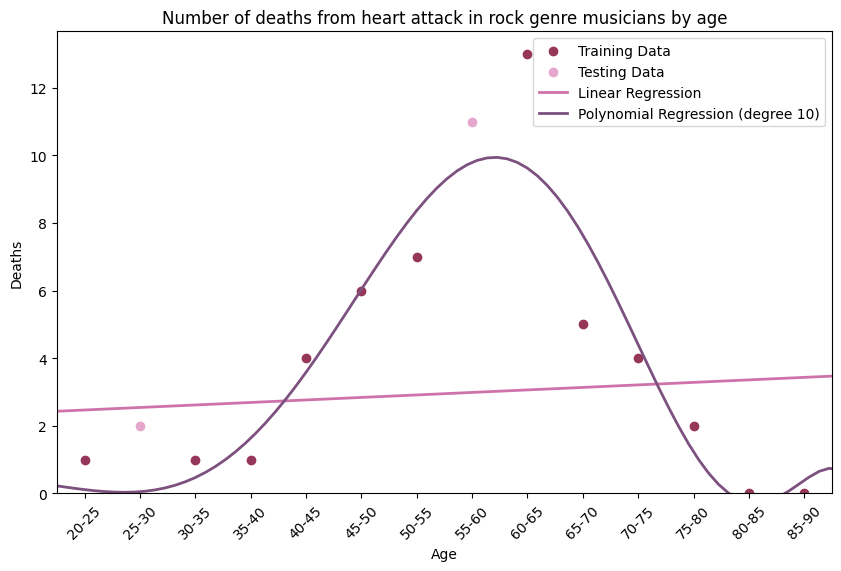
\includegraphics[width=0.6\linewidth]{graph_images/experiments/exp2.png}
    \label{fig:enter-label}
\end{figure}

\noindent\texttt{Linear Regression - Training Set: RMSE = 3.5293, R\textasciicircum2 = 0.0111\\
Linear Regression - Testing Set: RMSE = 4.3084, R\textasciicircum2 = 0.1027\\
Polynomial Regression - Training Set: RMSE = 1.2461, R\textasciicircum2 = 0.8767\\
Polynomial Regression - Testing Set: RMSE = 1.2231, R\textasciicircum2 = 0.9277\\}



\subsubsection{Fitting a linear regression model and a polynomial regression of degree n to the data: death cause - overdose, genre - hip hop}

\begin{figure} [H]
    \centering
    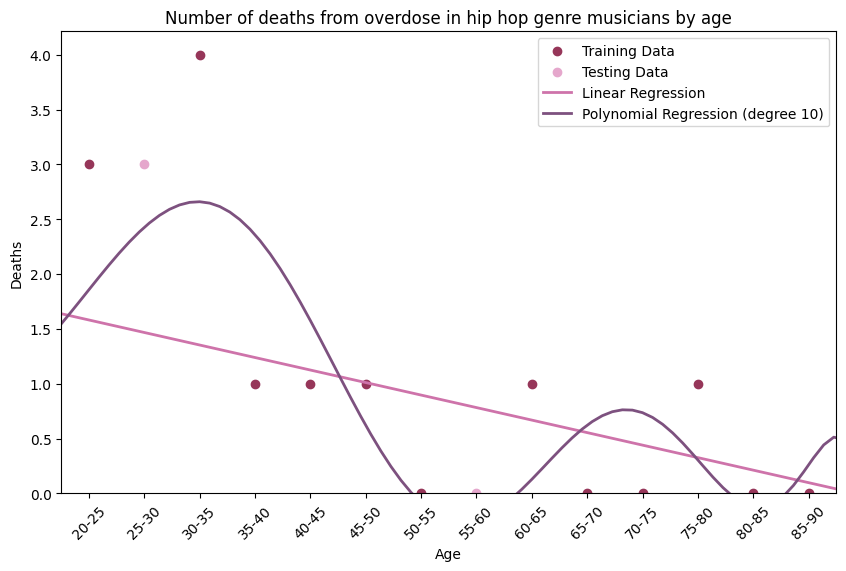
\includegraphics[width=0.6\linewidth]{graph_images/experiments/exp3.png}
    \label{fig:enter-label}
\end{figure}

\noindent\texttt{Linear Regression - Training Set: RMSE = 0.9924, R\textasciicircum2 = 0.2513\\
Linear Regression - Testing Set: RMSE = 1.6445, R\textasciicircum2 = -0.6026\\
Polynomial Regression - Training Set: RMSE = 0.7541, R\textasciicircum2 = 0.5677\\
Polynomial Regression - Testing Set: RMSE = 0.5984, R\textasciicircum2 = 0.7878\\}



\subsubsection{Fitting a linear regression model and a polynomial regression of degree n to the data: death cause - natural causes, genre - classical}

\begin{figure} [H]
    \centering
    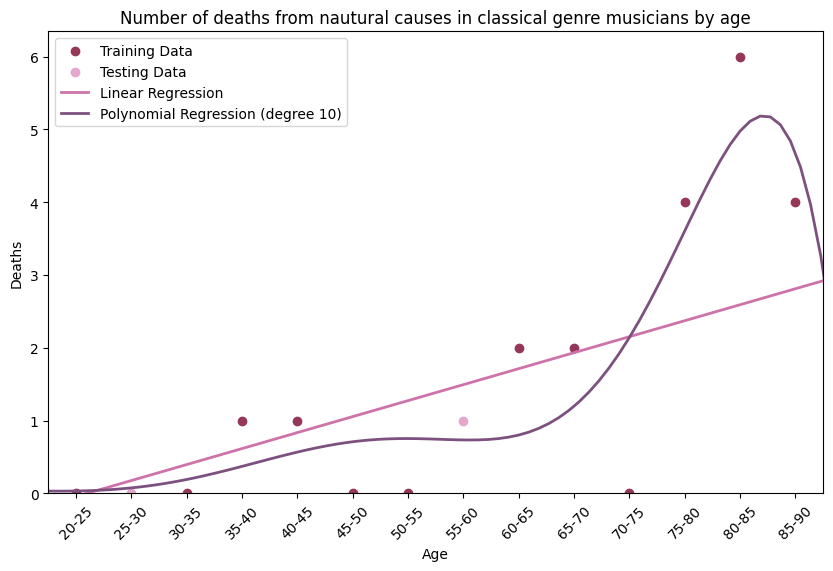
\includegraphics[width=0.6\linewidth]{graph_images/experiments/exp4.png}
    \label{fig:enter-label}
\end{figure}

\noindent\texttt{Linear Regression - Training Set: RMSE = 1.4823, R\textasciicircum2 = 0.358\\
Linear Regression - Testing Set: RMSE = 0.6359, R\textasciicircum2 = -1.1569\\
Polynomial Regression - Training Set: RMSE = 0.8183, R\textasciicircum2 = 0.8043\\
Polynomial Regression - Testing Set: RMSE = 0.1455, R\textasciicircum2 = 0.887\\}



\subsubsection{Fitting a linear regression model and a polynomial regression of degree n to the data: death cause - murder, skill - rapper}

\begin{figure} [H]
    \centering
    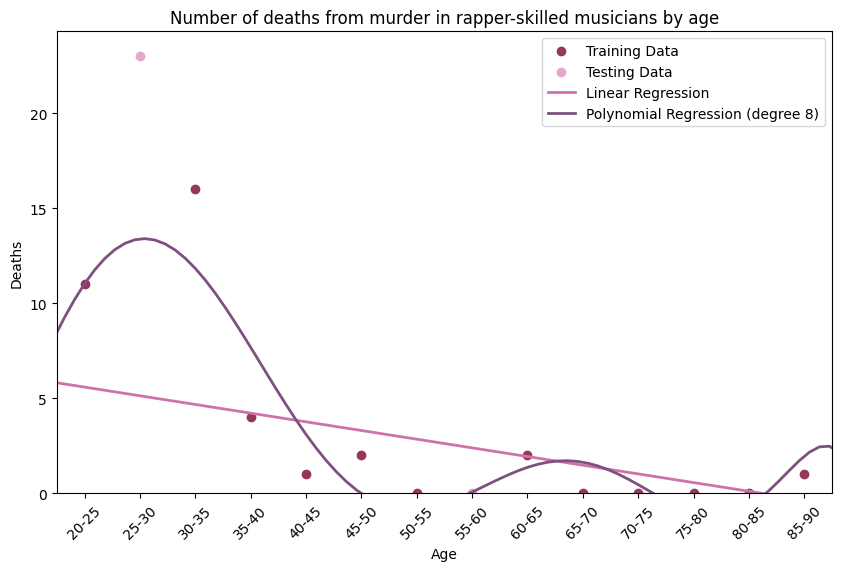
\includegraphics[width=0.6\linewidth]{graph_images/experiments/exp5.png}
    \label{fig:enter-label}
\end{figure}

\noindent\texttt{Linear Regression - Training Set: RMSE = 3.8946, R\textasciicircum2 = 0.2587\\
Linear Regression - Testing Set: RMSE = 10.3486, R\textasciicircum2 = -0.0797\\
Polynomial Regression - Training Set: RMSE = 1.7932, R\textasciicircum2 = 0.8429\\
Polynomial Regression - Testing Set: RMSE = 5.0576, R\textasciicircum2 = 0.7421\\}



\subsubsection{Fitting a linear regression model and a polynomial regression of degree n to the data: death cause - overdose, skill - rapper}

\begin{figure} [H]
    \centering
    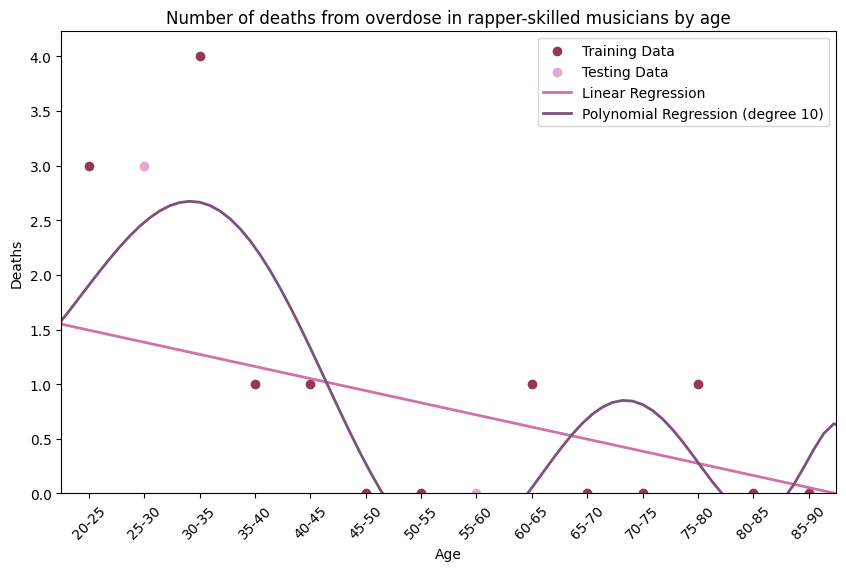
\includegraphics[width=0.6\linewidth]{graph_images/experiments/exp6.png}
    \label{fig:enter-label}
\end{figure}

\noindent\texttt{Linear Regression - Training Set: RMSE = 1.0239, R\textasciicircum2 = 0.2292\\
Linear Regression - Testing Set: RMSE = 1.5984, R\textasciicircum2 = -0.514\\
Polynomial Regression - Training Set: RMSE = 0.7494, R\textasciicircum2 = 0.5871\\
Polynomial Regression - Testing Set: RMSE = 0.6037, R\textasciicircum2 = 0.784\\}



\subsubsection{Fitting a linear regression model and a polynomial regression of degree n to the data: death cause - stroke, skill - vocals}

\begin{figure} [H]
    \centering
    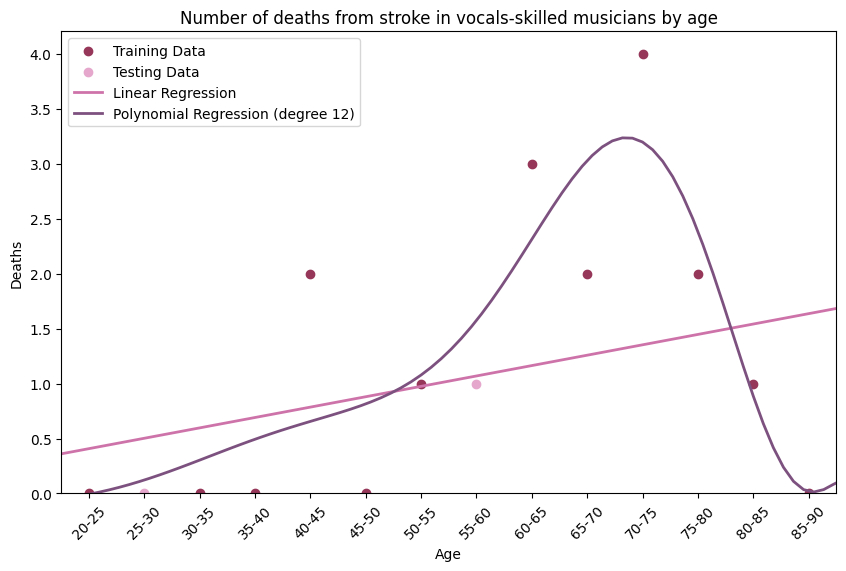
\includegraphics[width=0.6\linewidth]{graph_images/experiments/exp7.png}
    \label{fig:enter-label}
\end{figure}

\noindent\texttt{Linear Regression - Training Set: RMSE = 1.1718, R\textasciicircum2 = 0.1418\\
Linear Regression - Testing Set: RMSE = 0.2614, R\textasciicircum2 = 0.6355\\
Polynomial Regression - Training Set: RMSE = 0.5866, R\textasciicircum2 = 0.7849\\
Polynomial Regression - Testing Set: RMSE = 0.3019, R\textasciicircum2 = 0.5138\\}



\subsubsection{Fitting a linear regression model and a polynomial regression of degree n to the data: death cause - cancer, skill - guitar}

\begin{figure} [H]
    \centering
    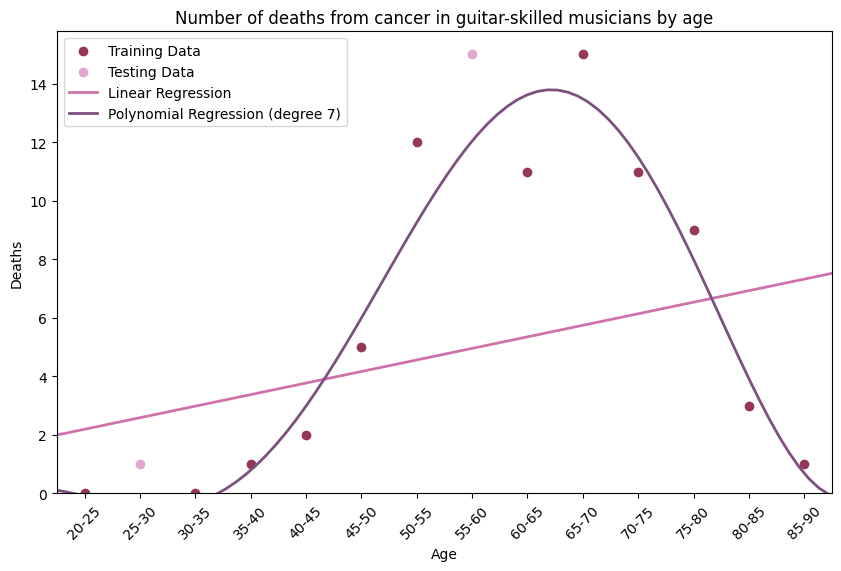
\includegraphics[width=0.6\linewidth]{graph_images/experiments/exp8.png}
    \label{fig:enter-label}
\end{figure}

\noindent\texttt{Linear Regression - Training Set: RMSE = 4.8028, R\textasciicircum2 = 0.1464\\
Linear Regression - Testing Set: RMSE = 5.1186, R\textasciicircum2 = 0.3531\\
Polynomial Regression - Training Set: RMSE = 1.1845, R\textasciicircum2 = 0.9481\\
Polynomial Regression - Testing Set: RMSE = 1.6843, R\textasciicircum2 = 0.93\\}




\section{Predictive model}
\subsection{Approach description}
After the experiments have been done, there was an attempt at creating a predictive model for the chances of dying to various causes, based on age and skills.

After some research, the \textit{SVC} algorithm was chosen to perform this task.

\textit{Support Vector Classification (SVC)} is a supervised learning algorithm used for classification tasks. It belongs to the family of Support Vector Machines (SVMs), which are powerful algorithms used for both classification and regression tasks.

The data has been properly categorized, encoded and split into training and testing sets. Then, the model has been fitted to the data and the probabilities were calculated using the \textit{predict\_proba} method. The classification report, containing performance indicators and support (column that indicates the number of instances of each class in the testing dataset), has then been generated using \textit{classification\_report} method.

The \textit{SVC }algorithm, \textit{predict\_proba} method and \textit{classification\_report} method were all taken from the scikit-learn library.

First constructed model predicts the probability of dying to two different death causes, based on age and skills provided by the user.
Second constructed model predicts the probability of dying to all available death causes, also based on user input.

The same model can be constructed for predictions based on genres. However, for demonstration purposes, I have chosen the skills dataset, since it has more data to base the model on.


\subsection{Sample results with performance evaluation scores}


\subsubsection{First model (two death causes)}

\begin{verbatim}
MODEL REPORT:
User input: age=60, musical_skill='drums', death_causes=['cancer', 'overdose']

Probabilities for age 60 and musical skill 'drums':
Probability of dying from cancer: 0.9313
Probability of dying from overdose: 0.0687

Training Accuracy: 0.9065420560747663
Testing Accuracy: 0.897196261682243

Classification Report:
              precision    recall  f1-score   support

      cancer       0.91      0.96      0.93        82
    overdose       0.85      0.68      0.76        25

    accuracy                           0.90       107
   macro avg       0.88      0.82      0.85       107
weighted avg       0.89      0.90      0.89       107



==============================================================================

MODEL REPORT:
User input: age=25, musical_skill='rapper', death_causes=['murder', 'natural causes']

Probabilities for age 25 and musical skill 'rapper':
Probability of dying from murder: 0.9183
Probability of dying from natural causes: 0.0817

Training Accuracy: 0.9233226837060703
Testing Accuracy: 0.8987341772151899

Classification Report:
                precision    recall  f1-score   support

        murder       0.85      0.65      0.73        17
natural causes       0.91      0.97      0.94        62

      accuracy                           0.90        79
     macro avg       0.88      0.81      0.84        79
  weighted avg       0.90      0.90      0.89        79


==============================================================================

MODEL REPORT:
User input: age=40, musical_skill='strings', death_causes=['cancer', 'heart attack']

Probabilities for age 40 and musical skill 'strings':
Probability of dying from cancer: 0.6272
Probability of dying from heart attack: 0.3728

Training Accuracy: 0.6343692870201096
Testing Accuracy: 0.6131386861313869

Classification Report:
              precision    recall  f1-score   support

      cancer       0.61      0.96      0.75        81
heart attack       0.67      0.11      0.18        56

    accuracy                           0.61       137
   macro avg       0.64      0.54      0.47       137
weighted avg       0.63      0.61      0.52       137

\end{verbatim}

\clearpage
\subsubsection{Second model (all death causes)}


\begin{verbatim}

MODEL REPORT:
User input: age=25, musical_skill='rapper'

Probabilities for age 25 and musical skill 'rapper':
Probability of dying from accident: 0.1637
Probability of dying from cancer: 0.015
Probability of dying from heart attack: 0.0565
Probability of dying from illness: 0.0537
Probability of dying from murder: 0.4348
Probability of dying from natural causes: 0.0212
Probability of dying from organ failure: 0.0434
Probability of dying from overdose: 0.1202
Probability of dying from stroke: 0.0163
Probability of dying from suicide: 0.0752

Training Accuracy: 0.27710144927536234
Testing Accuracy: 0.30324074074074076
Classification Report:
                precision    recall  f1-score   support

      accident       0.32      0.52      0.40        42
        cancer       0.26      0.86      0.40        79
  heart attack       1.00      0.00      0.00        51
       illness       0.00      0.00      0.00        88
        murder       0.41      0.50      0.45        24
natural causes       0.47      0.47      0.47        60
 organ failure       1.00      0.00      0.00        38
      overdose       1.00      0.00      0.00        24
        stroke       1.00      0.00      0.00         7
       suicide       0.17      0.05      0.08        19

      accuracy                           0.30       432
     macro avg       0.56      0.24      0.18       432
  weighted avg       0.45      0.30      0.20       432

==============================================================================

MODEL REPORT:
User input: age=70, musical_skill='guitar'

Probabilities for age 70 and musical skill 'guitar':
Probability of dying from accident: 0.0626
Probability of dying from cancer: 0.2549
Probability of dying from heart attack: 0.1498
Probability of dying from illness: 0.2174
Probability of dying from murder: 0.0214
Probability of dying from natural causes: 0.1129
Probability of dying from organ failure: 0.1093
Probability of dying from overdose: 0.0088
Probability of dying from stroke: 0.0452
Probability of dying from suicide: 0.0177

Training Accuracy: 0.27710144927536234
Testing Accuracy: 0.30324074074074076
Classification Report:
                precision    recall  f1-score   support

      accident       0.32      0.52      0.40        42
        cancer       0.26      0.86      0.40        79
  heart attack       1.00      0.00      0.00        51
       illness       0.00      0.00      0.00        88
        murder       0.41      0.50      0.45        24
...
      accuracy                           0.30       432
     macro avg       0.56      0.24      0.18       432
  weighted avg       0.45      0.30      0.20       432

==============================================================================

MODEL REPORT:
User input: age=45, musical_skill='drums'

Probabilities for age 45 and musical skill 'drums':
Probability of dying from accident: 0.2031
Probability of dying from cancer: 0.1767
Probability of dying from heart attack: 0.1116
Probability of dying from illness: 0.0975
Probability of dying from murder: 0.0282
Probability of dying from natural causes: 0.054
Probability of dying from organ failure: 0.134
Probability of dying from overdose: 0.0811
Probability of dying from stroke: 0.043
Probability of dying from suicide: 0.0707

Training Accuracy: 0.27710144927536234
Testing Accuracy: 0.30324074074074076
Classification Report:
                precision    recall  f1-score   support

      accident       0.32      0.52      0.40        42
        cancer       0.26      0.86      0.40        79
  heart attack       1.00      0.00      0.00        51
       illness       0.00      0.00      0.00        88
        murder       0.41      0.50      0.45        24
natural causes       0.47      0.47      0.47        60
 organ failure       1.00      0.00      0.00        38
      overdose       1.00      0.00      0.00        24
        stroke       1.00      0.00      0.00         7
       suicide       0.17      0.05      0.08        19

      accuracy                           0.30       432
     macro avg       0.56      0.24      0.18       432
  weighted avg       0.45      0.30      0.20       432


\end{verbatim}



\section{Conclusions}

The most obvious conclusion that can be drawn from the report is the importance of high-quality, varying data. The analysis seems to be very biased in all the areas that are lacking within the acquired dataset. However, with the right techniques, some dependencies and correlations could be clearly observed.

Regarding the linear and polynomial regression experiments, it was clear that the polynomial regression had the upper hand, resulting in much better performance indicator scores. However, in most cases, the degree of the polynomial had to be quite high (6-12). This might be the case due to the nature of the dataset - there isn't enough individual data and it is quite scattered across the graph.

Overall, the death age predictions during the experiments and death cause predictions made by the model have been somewhat of a success. 

When it comes to the predictive models, it has been observed that - on average - the first model has much better performance indicator scores. However, upon observation, the second model returns probabilities that seem to be matching with the provided dataset and can be observed in reality.

Age and musical skills appear to influence the likelihood of death causes among musicians, with certain genres and skills potentially associated with higher risks.

The predictive model demonstrates promising performance in forecasting death causes based on available attributes, although further refinement and more data may be necessary to improve accuracy, particularly for less prevalent causes.

Overall, the analyses and predictions provide valuable insights into the factors contributing to mortality among musicians and underscore the importance of considering various demographic and occupational factors in health-related research and interventions.


\section{References}

\begin{itemize}
    \item \textit{https://www.datacamp.com/tutorial/svm-classification-scikit-learn-python}
    \item \textit{https://musicbrainz.org/doc/MusicBrainz\_API}
    \item \textit{https://rateyourmusic.com/list/montezuma/all-dead-all-dead-worlds-largest-list-of-deceased-musicians/}
    \item \textit{https://www.geeksforgeeks.org/python-implementation-of-polynomial-regression/}
\end{itemize}

\end{document}